%package list
\documentclass{article}
\usepackage[top=3cm, bottom=3cm, outer=3cm, inner=3cm]{geometry}
\usepackage{multicol}
\usepackage{graphicx}
\usepackage{url}
%\usepackage{cite}
\usepackage{hyperref}
\usepackage{array}
%\usepackage{multicol}
\newcolumntype{x}[1]{>{\centering\arraybackslash\hspace{0pt}}p{#1}}
\usepackage{natbib}
\usepackage{pdfpages}
\usepackage{multirow}
\usepackage[normalem]{ulem}
\useunder{\uline}{\ul}{}
\usepackage{svg}
\usepackage{xcolor}
\usepackage{listings}
\lstdefinestyle{ascii-tree}{
    literate={├}{|}1 {─}{--}1 {└}{+}1 
  }
\lstset{basicstyle=\ttfamily,
  showstringspaces=false,
  commentstyle=\color{red},
  keywordstyle=\color{blue}
}
%\usepackage{booktabs}
\usepackage{caption}
\usepackage{subcaption}
\usepackage{float}
\usepackage{array}

\newcolumntype{M}[1]{>{\centering\arraybackslash}m{#1}}
\newcolumntype{N}{@{}m{0pt}@{}}


%%%%%%%%%%%%%%%%%%%%%%%%%%%%%%%%%%%%%%%%%%%%%%%%%%%%%%%%%%%%%%%%%%%%%%%%%%%%
%%%%%%%%%%%%%%%%%%%%%%%%%%%%%%%%%%%%%%%%%%%%%%%%%%%%%%%%%%%%%%%%%%%%%%%%%%%%
\newcommand{\itemEmail}{  \newline aanazcoh@unsa.edu.pe\newline  fvilcaqui@unsa.edu.pe \newline mhuamanivar@unsa.edu.pe \newline jturpoan@unsa.edu.pe}
\newcommand{\itemStudent}{Andre Renzo Añazco Huamanquispe\newline Frank's vilca Quispe\newline Melsy Melany Huamani Vargas \newline Jhamil Yeyder Turpo Añasco \newline}
\newcommand{\itemCourse}{Programación}
\newcommand{\itemCourseCode}{20231001}
\newcommand{\itemSemester}{III}
\newcommand{\itemUniversity}{Universidad Nacional de San Agustín de Arequipa}
\newcommand{\itemFaculty}{Facultad de Ingeniería de Producción y Servicios}
\newcommand{\itemDepartment}{Departamento Académico de Ingeniería de Sistemas e Informática}
\newcommand{\itemSchool}{Escuela Profesional de Ingeniería de Sistemas}
\newcommand{\itemAcademic}{2023 - A}
\newcommand{\itemInput}{Del 19 Junio 2023}
\newcommand{\itemOutput}{Al 19 Julio 2023}
\newcommand{\itemPracticeNumber}{05}
\newcommand{\itemTheme}{Django}
%%%%%%%%%%%%%%%%%%%%%%%%%%%%%%%%%%%%%%%%%%%%%%%%%%%%%%%%%%%%%%%%%%%%%%%%%%%%
%%%%%%%%%%%%%%%%%%%%%%%%%%%%%%%%%%%%%%%%%%%%%%%%%%%%%%%%%%%%%%%%%%%%%%%%%%%%

\usepackage[english,spanish]{babel}
\usepackage[utf8]{inputenc}
\AtBeginDocument{\selectlanguage{spanish}}
\renewcommand{\figurename}{Figura}
\renewcommand{\refname}{Referencias}
\renewcommand{\tablename}{Tabla} %esto no funciona cuando se usa babel
\AtBeginDocument{%
	\renewcommand\tablename{Tabla}
}

\usepackage{fancyhdr}
\pagestyle{fancy}
\fancyhf{}
\setlength{\headheight}{30pt}
\renewcommand{\headrulewidth}{1pt}
\renewcommand{\footrulewidth}{1pt}
\fancyhead[L]{\raisebox{-0.2\height}{
\includegraphics[width=3cm]{img/logo_episunsa.png}}}
\fancyhead[C]{\fontsize{7}{7}\selectfont	\itemUniversity \\ \itemFaculty \\ \itemDepartment \\ \itemSchool \\ \textbf{\itemCourse}}
\fancyhead[R]{\raisebox{-0.2\height}{
\includegraphics[width=1.2cm]{img/logo_abet}}}
\fancyfoot[L]{Estudiante Juan Perez Perez}
\fancyfoot[C]{\itemCourse}
\fancyfoot[R]{Página \thepage}

% para el codigo fuente
\usepackage{listings}
\usepackage{color, colortbl}
\definecolor{dkgreen}{rgb}{0,0.6,0}
\definecolor{gray}{rgb}{0.5,0.5,0.5}
\definecolor{mauve}{rgb}{0.58,0,0.82}
\definecolor{codebackground}{rgb}{0.95, 0.95, 0.92}
\definecolor{tablebackground}{rgb}{0.8, 0, 0}

\lstset{frame=tb,
	language=bash,
	aboveskip=3mm,
	belowskip=3mm,
	showstringspaces=false,
	columns=flexible,
	basicstyle={\small\ttfamily},
	numbers=none,
	numberstyle=\tiny\color{gray},
	keywordstyle=\color{blue},
	commentstyle=\color{dkgreen},
	stringstyle=\color{mauve},
	breaklines=true,
	breakatwhitespace=true,
	tabsize=3,
	backgroundcolor= \color{codebackground},
}

\begin{document}
	
	\vspace*{10px}
	
	\begin{center}	
		\fontsize{17}{17} \textbf{ Informe de Laboratorio \itemPracticeNumber}
	\end{center}
	\centerline{\textbf{\Large Tema: \itemTheme}}
	%\vspace*{0.5cm}	

	\begin{flushright}
		\begin{tabular}{|M{2.5cm}|N|}
			\hline 
			\rowcolor{tablebackground}
			\color{white} \textbf{Nota}  \\
			\hline 
			     \\[30pt]
			\hline 			
		\end{tabular}
	\end{flushright}	

	\begin{table}[H]
		\begin{tabular}{|x{4.7cm}|x{4.8cm}|x{4.8cm}|}
			\hline 
			\rowcolor{tablebackground}
			\color{white} \textbf{Estudiante} & \color{white}\textbf{Escuela}  & \color{white}\textbf{Asignatura}   \\
			\hline 
			{\itemStudent \par \itemEmail} & \itemSchool & {\itemCourse \par Semestre: \itemSemester \par Código: \itemCourseCode}     \\
			\hline 			
		\end{tabular}
	\end{table}		
	
	\begin{table}[H]
		\begin{tabular}{|x{4.7cm}|x{4.8cm}|x{4.8cm}|}
			\hline 
			\rowcolor{tablebackground}
			\color{white}\textbf{Laboratorio} & \color{white}\textbf{Tema}  & \color{white}\textbf{Duración}   \\
			\hline 
			\itemPracticeNumber & \itemTheme & 04 horas   \\
			\hline 
		\end{tabular}
	\end{table}
	
	\begin{table}[H]
		\begin{tabular}{|x{4.7cm}|x{4.8cm}|x{4.8cm}|}
			\hline 
			\rowcolor{tablebackground}
			\color{white}\textbf{Semestre académico} & \color{white}\textbf{Fecha de inicio}  & \color{white}\textbf{Fecha de entrega}   \\
			\hline 
			\itemAcademic & \itemInput &  \itemOutput  \\
			\hline 
		\end{tabular}
	\end{table}
	
	\section{Tarea}
	\begin{itemize}		
		\item Implementar el algoritmo de ordenamiento por inserción en Java para mostrar el comportamiento de su complejidad para el peor caso.
		\item Utilizar Git para evidenciar su trabajo.
		\item Enviar trabajo al profesor en un repositorio GitHub Privado, dándole permisos como colaborador.
	\end{itemize}
		
	\section{Equipos, materiales y temas utilizados}
	\begin{itemize}
		\item Sistema Operativo Ubuntu GNU Linux 23 lunar 64 bits Kernell 6.2.
		\item VIM 9.0.
		\item OpenJDK 64-Bits 17.0.7.
		\item Git 2.39.2.
		\item Cuenta en GitHub con el correo institucional.
		\item Programación Orientada a Objetos.
		\item Algoritmo de ordenamiento por inserción	
	\end{itemize}
	
	\section{URL de Repositorio Github}
	\begin{itemize}
		\item URL del Repositorio GitHub para clonar o recuperar.
		\item \url{https://github.com/rescobedoq/programacion.git}
		\item URL para el laboratorio 01 en el Repositorio GitHub.
		\item \url{https://github.com/rescobedoq/programacion/tree/main/lab01}
	\end{itemize}
	
	\section{Actividades con el repositorio GitHub}
	
	\subsection{Creando e inicializando repositorio GitHub}
	\begin{itemize}	
		\item Como es el primer laboratorio se creo el repositorio GitHub.
		\item Se realizaron los siguientes comandos en la computadora:
	\end{itemize}	
		
	\begin{lstlisting}[language=bash,caption={Creando directorio de trabajo}][H]
		$ mkdir -p $HOME/rescobedoq/
	\end{lstlisting}
	\begin{lstlisting}[language=bash,caption={Dirijíéndonos al directorio de trabajo}][H]
		$ cd $HOME/rescobedoq/
	\end{lstlisting}	
	\begin{lstlisting}[language=bash,caption={Creando directorio para repositorio GitHub}][H]
		$ mkdir -p $HOME/rescobedoq/programacion
	\end{lstlisting}
	\begin{lstlisting}[language=bash,caption={Inicializando directorio para repositorio GitHub}][H]
		$ cd $HOME/rescobedoq/programacion
		$ echo "# programacion" >> README.md
		$ git init
		$ git config --global user.name "Richart Smith Escobedo Quispe"
		$ git config --global user.email rescobedoq@gmail.com
		$ git add README.md
		$ git commit -m "first commit"
		$ git branch -M main
		$ git remote add origin https://github.com/rescobedoq/programacion.git
		$ git push -u origin main
	\end{lstlisting}
	
	\subsection{Commits}
	\begin{lstlisting}[language=bash,caption={Primer Commit Creando carpeta/archivo para laboratorio 01}][H]
		$ mkdir lab01
		$ touch lab01/Insertion.java
		$ git add .
		$ git commit -m "Creando carpeta/archivo para laboratorio 01"			
		$ git push -u origin main
	\end{lstlisting}
	
	\begin{itemize}	
		\item Se creo el archivo \textbf{.gitignore} para no considerar los archivos \textbf{*.class} que son innecesarios hacer seguimiento.
	\end{itemize}
	\begin{lstlisting}[language=bash,caption={Creando .gitignore}][H]
		$ vim lab01/.gitignore
	\end{lstlisting}
	\begin{lstlisting}[language=bash,caption={lab01/.gitignore}][H]
		*.class
	\end{lstlisting}
	\begin{lstlisting}[language=bash,caption={Commit: Creando .gitignore para archivos *.class}][H]
		$ git add .
		$ git commit -m "Creando .gitignore para archivos *.class"			
		$ git push -u origin main
	\end{lstlisting}
	
	\begin{itemize}	
		\item Para el siguiente commit se implemento el algoritmo de ordenamiento por Inserción, se imprime el arreglo caso definido en el mismo código.
		\item El pseudocódigo utilizado es el siguiente:
	\end{itemize}	
	
	\begin{figure}[H]
		\centering
		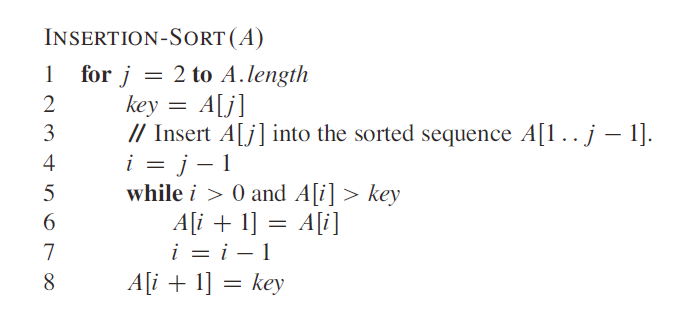
\includegraphics[width=0.8\textwidth,keepaspectratio]{img/pseudocodigo_insercion.png}
		%\includesvg{img/automata.svg}
		%\label{img:mot2}
		%\caption{Product backlog.}
	\end{figure}
	
	\clearpage
	
	\begin{lstlisting}[language=bash,caption={Creando .gitignore}][H]
		$ vim lab01/Insertion.java
	\end{lstlisting}
	
	\lstinputlisting[language=Java, caption={Insertion.java},numbers=left,]{src/Insertion01.java}
	
	\begin{lstlisting}[language=bash,caption={Compilando y probando código}][H]
		$ cd lab01
		$ javac Insertion.java
		$ java Insertion
		5 2 4 6 1 3 
		5 5 4 6 1 3 
		2 5 5 6 1 3 
		2 4 5 6 1 3 
		2 2 4 5 6 3 
		1 2 4 4 5 6
	\end{lstlisting}
	\begin{lstlisting}[language=bash,caption={Commit: Probando algoritmo de Inserción con arreglo}][H]
		$ git add .
		$ git commit -m "Probando algoritmo de Insercion con arreglo"			
		$ git push -u origin main
	\end{lstlisting}
	
		
	\subsection{Estructura de laboratorio 01}
	\begin{itemize}	
		\item El contenido que se entrega en este laboratorio es el siguiente:
	\end{itemize}
	
\begin{lstlisting}[style=ascii-tree]
lab01/
|--- Insertion.java
|--- latex
    |--- img
    |   |--- logo_abet.png
    |   |--- logo_episunsa.png
    |   |--- logo_unsa.jpg
    |   |--- pseudocodigo_insercion.png    
    |--- programacion_lab01_rescobedoq_v1.0.pdf    
    |--- programacion_lab01_rescobedoq_v1.0.tex
    |--- src
        |--- Insertion01.java
\end{lstlisting}    

\section{Pregunta: ¿Cúal es el comportamiento del algoritmo de ordenamiento por inserción?}
	\begin{itemize}
		\item El algoritmo muestra un comportamiento cuadrático de O(n²).
		\item Se trabajarón los peores casos desde una arreglo de tamaño 1 hasta N.
		\item Para obtener un grafico ideal se utilizó N=10,000.
	\end{itemize}		

	\section{\textcolor{red}{Rúbricas}}
	
	\subsection{\textcolor{red}{Entregable Informe}}
	\begin{table}[H]
		\caption{Tipo de Informe}
		\setlength{\tabcolsep}{0.5em} % for the horizontal padding
		{\renewcommand{\arraystretch}{1.5}% for the vertical padding
		\begin{tabular}{|p{3cm}|p{12cm}|}
			\hline
			\multicolumn{2}{|c|}{\textbf{\textcolor{red}{Informe}}}  \\
			\hline 
			\textbf{\textcolor{red}{Latex}} & \textcolor{blue}{El informe está en formato PDF desde Latex,  con un formato limpio (buena presentación) y facil de leer.}   \\ 
			\hline 
			
			
		\end{tabular}
	}
	\end{table}
	
	\clearpage
	
	\subsection{\textcolor{red}{Rúbrica para el contenido del Informe y demostración}}
	\begin{itemize}			
		\item El alumno debe marcar o dejar en blanco en celdas de la columna \textbf{Checklist} si cumplio con el ítem correspondiente.
		\item Si un alumno supera la fecha de entrega,  su calificación será sobre la nota mínima aprobada, siempre y cuando cumpla con todos lo items.
		\item El alumno debe autocalificarse en la columna \textbf{Estudiante} de acuerdo a la siguiente tabla:
	
		\begin{table}[ht]
			\caption{Niveles de desempeño}
			\begin{center}
			\begin{tabular}{ccccc}
    			\hline
    			 & \multicolumn{4}{c}{Nivel}\\
    			\cline{1-5}
    			\textbf{Puntos} & Insatisfactorio 25\%& En Proceso 50\% & Satisfactorio 75\% & Sobresaliente 100\%\\
    			\textbf{2.0}&0.5&1.0&1.5&2.0\\
    			\textbf{4.0}&1.0&2.0&3.0&4.0\\
    		\hline
			\end{tabular}
		\end{center}
	\end{table}	
	
	\end{itemize}
	
	\begin{table}[H]
		\caption{Rúbrica para contenido del Informe y demostración}
		\setlength{\tabcolsep}{0.5em} % for the horizontal padding
		{\renewcommand{\arraystretch}{1.5}% for the vertical padding
		%\begin{center}
		\begin{tabular}{|p{2.7cm}|p{7cm}|x{1.3cm}|p{1.2cm}|p{1.5cm}|p{1.1cm}|}
			\hline
    		\multicolumn{2}{|c|}{Contenido y demostración} & Puntos & Checklist & Estudiante & Profesor\\
			\hline
			\textbf{1. GitHub} & Hay enlace URL activo del directorio para el  laboratorio hacia su repositorio GitHub con código fuente terminado y fácil de revisar. &2 &X &2 & \\ 
			\hline
			\textbf{2. Commits} &  Hay capturas de pantalla de los commits más importantes con sus explicaciones detalladas. (El profesor puede preguntar para refrendar calificación). &4 & & & \\ 
			\hline 
			\textbf{3. Código fuente} &  Hay porciones de código fuente importantes con numeración y explicaciones detalladas de sus funciones. &2 &X &2 & \\ 
			\hline 
			\textbf{4. Ejecución} & Se incluyen ejecuciones/pruebas del código fuente  explicadas gradualmente. &2 &X &2 & \\ 
			\hline			
			\textbf{5. Pregunta} & Se responde con completitud a la pregunta formulada en la tarea.  (El profesor puede preguntar para refrendar calificación).  &2 &X &2 & \\ 
			\hline	
			\textbf{6. Fechas} & Las fechas de modificación del código fuente estan dentro de los plazos de fecha de entrega establecidos. &2 &X &2 & \\ 
			\hline 
			\textbf{7. Ortografía} & El documento no muestra errores ortográficos. &2 &X &2 & \\ 
			\hline 
			\textbf{8. Madurez} & El Informe muestra de manera general una evolución de la madurez del código fuente,  explicaciones puntuales pero precisas y un acabado impecable.   (El profesor puede preguntar para refrendar calificación).  &4 & & & \\ 
			\hline
			\multicolumn{2}{|c|}{\textbf{Total}} &20 & &12 & \\ 
			\hline
		\end{tabular}
		%\end{center}
		%\label{tab:multicol}
		}
	\end{table}
	
\clearpage

\section{Referencias}
\begin{itemize}			
	\item \url{https://www.w3schools.com/java/default.asp}
	\item \url{https://www.geeksforgeeks.org/insertion-sort/}
\end{itemize}	
	
%\clearpage
%\bibliographystyle{apalike}
%\bibliographystyle{IEEEtranN}
%\bibliography{bibliography}
			
\end{document}